\documentclass[12pt]{article}
\usepackage{graphicx}
\usepackage{booktabs}
\usepackage[margin=1.0in]{geometry}
\usepackage{color}
\usepackage{xcolor,tikz} %% for boxes in images
\usepackage{tabularx}
%Times New Roman 12 pt
\usepackage[T1]{fontenc}
\usepackage{mathptmx}
\usepackage{amssymb}
\usepackage{amsmath}
\usepackage{subcaption}
\usepackage{authblk}
\usepackage[backend=bibtex,style=phys]{biblatex}

\graphicspath{{snapshots/},{flexible/},{rigid/}}

\captionsetup{font=footnotesize,labelfont=footnotesize,skip=0pt,labelfont=bf}
\captionsetup[sub]{font=footnotesize,labelfont=footnotesize,skip=0pt,labelfont=bf}


% commands for paper
\newcommand\crule[3][black]{\textcolor{#1}{\rule{#2}{#3}}}
%\newcommand\mybox[2][]{\tikz[overlay]\node[fill=black,inner sep=2pt,text color=white,rectangle,#1] {#2};\phantom{#2}} % anchor=text, 
\newcommand{\angstrom}{\textup{\AA}}

\title{}
\author[1]{Lisa E. Felberg}
\author[2]{Luis A. Ruiz Pestana} 
\author[1-4]{Teresa Head-Gordon} 

\addbibresource{references}

\affil[1]{Department of Chemical and Biomolecular Engineering, University of California Berkeley, 
Berkeley, California 94720, USA}
\affil[2]{Chemical Sciences Division, Lawrence Berkeley National Labs
Berkeley, California 94720, USA}
\affil[3]{Department of Chemistry, University of California Berkeley, 
Berkeley, California 94720, USA}
\affil[4]{Department of Bioengineering, University of California Berkeley, 
Berkeley, California 94720, USA}


\date{}
\setcounter{Maxaffil}{0}
\renewcommand\Affilfont{\itshape\small}

\begin{document}
	\maketitle
\clearpage

\section*{Abstract}

\clearpage

%%%%%%%%%%%%%%%%%%%%%%%%%%%%%%%%%%%%%%%%
%%%%%%%%%%%%%%%%%%%%%%%%%%%%%%%%%%%%%%%%
%%%%%%%%%%%%%%%%%%%%%%%%%%%%%%%%%%%%%%%%
\section*{Introduction}

The properties and phase behavior of water under nanoconfinement are remarkably different than those in bulk, with important implications for nanotechnological applications and biological processes \cite{Lucent2007, Holt2006, Levinger2002, Nair2012}. Driven by the pursuit to understand the physics underlying the anomalous behavior of water under hydrophobic nanoconfinement, topics such as low-dimensional ice formation \cite{Algara-Siller2015, Koga2001} (which remains controversial \cite{Zhou2015}), unconventional solid-liquid and liquid-liquid phase transitions  \cite{Mochizuki2015,Han2010,Giovambattista2009,Zhu2015}, or hydrophobic evaporation (i.e. liquid-gas phase transitions) \cite{Sharma2012,Altabet2017,Head-Gordon2008,Hummer2001}, have been extensively studied over the last decade. It is important to note that the literature on confined water is vast, and the references cited in this letter are representative, but by no means exhaustive. 

When water is confined under slit nanocapillaries, such as in between graphene sheets, it exhibits strong density fluctuations in the direction of confinement, signature of a layered structure. The surface effect persists to distances of about 5 \r A \cite{Cicero2008,Chialvo2016}, suggesting that configurations of up to three layers of water should be stable under planar confinement. Indeed, multilayered ice phases up to trilayers have been observed \cite{Algara-Siller2015,Satarifard2017}. A requirement to form crystalline arrangements, besides low temperatures or high confinement pressures (in the order of GPa at room temperature \cite{Algara-Siller2015,Satarifard2017}), is that the confinement distance and the amount of water are commensurate, i.e. the density of water is such that individual layers can develop in-plane long-range order \cite{Satarifard2017,Chen2017,Corsetti2016}. When the density is too high or two low, all other control parameters constant, the confinement becomes incommensurate, the water cannot develop long-range in-plane order, and more disordered phases prevail. In the case of a monolayer, before the transition from ice to a liquid phase \cite{Han2010}, a puckered configuration forms \cite{Kaneko2014,Zhu2016}. The solid-liquid phase transition triggered by incommensurability is also observed for other multilayered phases of ice \cite{Zhu2015}. Interestingly, at higher temperatures or lower pressures where liquid phases are more stable, liquid-liquid transitions are also triggered by differences in commensurability. For example, a transition between a bilayer liquid phase and a trilayer heterogeneous fluid, as the density was increased, has been reported \cite{Giovambattista2009}. The heterogeneous liquid consists of a layered structure with relatively highly ordered layers close to the confining surfaces, and a highly disordered intermediate layer. A recent study where oscillations in the shear viscosity of confined water of several orders of magnitude where observed over changes in the confinement distance as small as one \r Angstrom \cite{Neek-Amal2016}, is another example of the significant effect of commensurability in confined systems.

What these studies have in common is the use of rigid confining surfaces, even when graphene in employed. Graphene is a two-dimensional carbon allotrope, intrinsically flexible \cite{Wei2013,Fasolino2007}, that due its unique properties \cite{Geim2007} has become a paradigmatic example of hydrophobic confining surface. Only a few studies have considered flexible confining surfaces, and the reported differences with respect to rigid confinement depend on the simulation conditions and system setup: from insignificant effects observed on the structure single-layer square ice formed by a small pocket of water confined between much larger graphene sheets \cite{Algara-Siller2015}, to relatively mild effects on structural and dynamical properties of water confined by multilayered free standing graphene systems \cite{Deshmukh2014}, to changes of many orders of magnitude in the hydrophobic evaporation rate when flexible graphene-like walls clamped at the ends are used \cite{Altabet2017}. Given the complex phase behavior of confined water, and the sensitivity to certain control parameters and system setup, there is a crucial gap in our fundamental understanding of confined water: Does the phase behavior of water mapped under rigid confinement extend to the more realistic conditions of flexible confinement?

Here, we study the phase behavior of confined water under physically accurate flexible graphene sheets using molecular dynamics simulations at constant ambient temperature and pressure. We find that when the system is commensurate, the flexibility of the confining surfaces has only marginal effects on the phase behavior, justifying the use of rigid models to study commensurate configurations, such as ice phases. On the other hand, the flexibility of graphene has a tremendous impact on incommensurate configurations, where the graphene sheets bend to accommodate a novel biphasic layered state, where an n-layer and an (n+1)-layer phase coexist next to each other. This multiphase coexisting state is reminiscent of that observed under inhomogeneous confinement \cite{Qiu2015}, with the important difference that here the inhomogeneity is not enforced, but self-imposed by the system. When the same incommensurate systems are simulated under rigid confinement, disordered liquid phases, similar to the heterogeneous fluid described above, are observed. The biphasic multilayer state under flexible confinement persists across a relatively wide range of confining distances. We observe biphasic states at incommensurate confinement distances where 0 and 1, 1 and 2, and 2 and 3, layered phases coexist. The regions with water in the 0/1 state form ice domains with both rhombic and distorted-square lattices. Remarkably, increasing the temperature of the system can trigger the transition from the biphasic liquid state to the heterogeneous fluid phase. This study provides new comprehensive understanding of the phase behavior of confined water, and sheds light into the role of flexible confinement and its interplay with commensurability effects. Furthermore, our results, based on a realistic model of graphene, will be useful to interpret experimental results in the future, where carbon allotropes are ubiquitously employed.

%%%%%%%%%%%%%%%%%%%%%%%%%%%%%%%%%%%%%%%%
%%%%%%%%%%%%%%%%%%%%%%%%%%%%%%%%%%%%%%%%
%%%%%%%%%%%%%%%%%%%%%%%%%%%%%%%%%%%%%%%%
\section*{Methods}

\textit{Models:} For this study, simulations of systems with parallel graphene plates with
separations of 6 and 12 \r A respectively in the x-cartesian dimension.
Systems of two different sizes were used to explore periodic size effects, with graphene
plate separation held constant. The systems had y-z dimensions of 46.2 by 48.5 \r A.

\textit{Force fields:} Harmonic bond and angle potentials were applied to the graphene sheets with 
the following parameters: k\textsubscript{bond} = 938.0 \(kCal/mol/\angstrom^2\)
and k\textsubscript{angle} = 126.0 \(kCal/mol/rad^2\), equilibrium bond and 
angle lengths of 1.40 \r A and 120.0 degrees respectively \cite{Hummer2001}. The
dihedral potential is harmonic with the functional form: \(E_{\text{di}} = K_{\text{di}} [ 1 + d cos(\phi)]\),
where K\textsubscript{di} = 3.15 kCal/mol, \(\phi = 180.0\) degrees and \(d = \pm 1\) \cite{Patra2009}. An improper torsional 
potential with a harmonic functional form as follows: \( E_{\text{im}} = K_{\text{im}} [ \chi - \chi_0 ]^2\) was
used with parameters K\textsubscript{im} =  15.0 kCal/mol and \(\chi_0 = 0.0\) degrees. A summary
of these potentials and their parameter values are given in Table \ref{table:ff_parms}
The water model chosen is TIP4P-Ew \cite{Horn2004} was used 
to represent explicit solvent. Partial charges and Van der Waals parameters for each atom type 
are given in Table \ref{table:ff_parms_atoms}.

\begin{table}[ht!]
\centering
\begin{tabular}{ lllll } \hline
Bond     &         & \(K_b\)  (\(kCal/mol/\angstrom^2\))      & b\textsubscript{0}  (\r A)            &          \\ \hline
         & C-C     & 938.0         & 1.40            &          \\
         &         &               &                 &          \\ \hline
Angle    &         & \(K_{\theta}\)  (\(kCal/mol/rad^2\)) & \(\theta_0\) (degrees)   &          \\ \hline
         & C-C-C   & 126.0         & 120.0           &          \\
                           &         &               &                 &          \\ \hline
Improper &         & K\textsubscript{im} (kCal/mol)       & \(\chi_0\) (degrees)     &          \\ \hline
         & C-C-C-C & 15.0          & 0.0             &          \\
                           &         &               &                 &          \\ \hline
Dihedral &         & K\textsubscript{di} (kCal/mol)       & n (multiplicity) & \(\phi\) (degrees)\\ \hline
         & C-C-C-C & 3.150         & 2               & 180.0  \\ 
\end{tabular}
\caption{\textit{Force field bonded parameters used for graphene in confined water simulations.}}
\label{table:ff_parms}
\end{table}

\begin{table}[ht!]
\centering
\begin{tabular}{|c|r|r|r|}
\hline
\textbf{Atom type} & \multicolumn{1}{c|}{\textbf{\begin{tabular}[c]{@{}c@{}}Partial charge\\ (e)\end{tabular}}} & \multicolumn{1}{c|}{\textbf{\begin{tabular}[c]{@{}c@{}}\(\sigma\)\\ (\r A)\end{tabular}}} & \multicolumn{1}{c|}{\textbf{\begin{tabular}[c]{@{}c@{}}\(\epsilon\)\\ (kCal/mole)\end{tabular}}} \\ \hline
Graphene carbon    & 0.0000                                                                                     & 3.55000                                                                              & 0.07000                                                                                     \\ \hline
Water oxygen       & -1.0484                                                                                    & 3.16435                                                                              & 0.16275                                                                                     \\ \hline
Water hydrogen     & 0.5242                                                                                     & 0.00000                                                                              & 0.00000                                                                                     \\ \hline
\end{tabular}
\caption{\textit{Force field parameters used for each atom type in confined water simulations.}}
\label{table:ff_parms_atoms}
\end{table}

\textit{Simulation protocols:} Simulations were performed with the LAMMPS software package \cite{Plimpton1995}. 
Equilibration of initial configurations were performed as follows. Systems were run in 
the NVE ensemble with a Langevin Thermostat at 298 Kelvin
for 10 ps. The water was then fixed with the SHAKE protocol \cite{Andersen1983} with a tolerance
of 10\textsuperscript{-4} and the system was run for 10 ps in the NVT ensemble.
Finally, data was saved for analysis in a production run in the NpT ensemble,
during which all cartesian coordinates were stored every 500 timesteps. 
Systems were run in the NpT ensemble for 10 ns. The 
pressure in the direction orthogonal to the graphene walls was maintained at 1 atm.
Thermal and pressure control were implemented using a Nos\' e-Hoover 
extended Lagrangian procedure \cite{Martyna1994} with characteristic damping times of 100 
and 1000 fs (0.1 and 1.0 ps), respectively. The dynamical integration 
scheme was velocity-Verlet \cite{Swope1982}.
For all simulations, the dynamics timestep was set at 2.0 femtoseconds. 

\textit{Analysis:} For the analysis, the first 3 nanoseconds of each trajectory was discarded and quantitative system properties were calculated and averaged over 3500 snapshots. Lateral pair correlation functions (g(R)s) between water oxygens were computed. The confining scale was in many instances comparable to the distance scale of water pair interaction lengthscales, therefore instead of computing a traditional 3D g(R), a lateral, or 2D, g(R) was computed as follows: water oxygens were histogrammed into 0.6\r A bins according to their x axis position (the graphene sheets fall in the y-z plane). Oxygens identified to be in the same bin were used to calculate a pair-correlation function, which was averaged for all bins. 3-body angle distributions were computed to analyze the in-plane water structure as follows. Like the lateral g(R)s, the oxygen atoms were binned according to their x-axis positions and then the two nearest neighbors were found for each oxygen. The angle computed is formed between the closest neighboring oxygen, the oxygen itself and the second closest neighbor. Graphene-graphene distances and water-graphene distances were considered to understand the effect of the flexible walls as well as to calculate the out-of-plane distribution of waters between the walls. For simplicity, the position of the waters was calculated with respect to a reference wall (one of the two in the simulation box), by considering the distance to the water oxygen. Finally, mean square displacement (MSD) calculations of water oxygens were made performing a sliding window, to allow for more statistics to be collected. For each timestep,\textit{t}, each atom was moved into the periodic image closest to itself in the previous timestep, \textit{t-1}, to ensure that the effects of the periodic boundary conditions were corrected for. The center of mass was the computed for the unwrapped coordinates and this center was subtracted from each atom to account for the effect of collective movement. In this way, displacement in each dimension was computed, but for an estimation of the diffusion coefficient, \(\mathcal{D}_{||}\), MSD in the dimension parallel to the graphene sheets was considered (MSD\textsubscript{||}). The slope of MSD\textsubscript{||} versus time, \textit{m}, was calculated, and \(\mathcal{D}_{||}\) was computed according to the Einstein relation: \(\mathcal{D}_{||}\) = 4\textit{m}.

%%%%%%%%%%%%%%%%%%%%%%%%%%%%%%%%%%%%%%%%
%%%%%%%%%%%%%%%%%%%%%%%%%%%%%%%%%%%%%%%%
%%%%%%%%%%%%%%%%%%%%%%%%%%%%%%%%%%%%%%%%
\subsection*{Results}

All the systems studied here, both rigid and flexible, are simulated at room temperature and pressure. The only prescribed parameter for each system is the 2D density of water, \(\rho_{2D}\), calculated as the number of water molecules per interlayer divided by the area of the graphene sheet. This way we avoid making ambiguous measurements of the 3D density under confinement, which requires choosing an ill-defined excluded distance from the confining surfaces. The values of \(\rho_{2D}\), which span from 0.097 to 0.390, are chosen such that we can sample systems that range from an incomplete single layer to systems where 3 full layers can form, and everything in between.

\textit{Layering}. The out-of-plane phase behavior, or layering, is illustrated in Figure \ref{fig:dgg_1} that shows the dependence of the confining distance, \(d_{gg}\) on \(\rho_{2D}\), for both flexible and rigid cases. We observe three regimes characterized by minimal changes of \(d_{gg}\) with \(\rho_{2D}\), alternated by first-order phase transitions marked by abrupt changes in \(d_{gg}\). \textcolor{red}{LF note: It was marked here that the transition in spacing has been observed before, but in my readings, most simulations maintain a fixed graphene separation, so I don't know if this has been seen.} In the case of flexible confinement, the phase transition occurs at the same values of \(\rho_{2D}\) as for the rigid case, but the transition is qualitatively different. We observe a split in the \(d_{gg}\) distances, which corresponds to the simultaneous coexistence of a n-layer and an (n+1)-layer phases in the same system. The snapshots shown in Figure \ref{fig:dgg_2} (left panels) illustrate this coexistence, where each phase occupies a distinct region of the system.

When comparing transitions between layers in the rigid system, there is a distinct difference observed in transitions from 1 to 2 interlayers and the transition from 2 layers to 3 and beyond. For the systems studied there is a clustering of monolayer systems for both the flexible and rigid cases where independent of the 2D density, the graphene-graphene separation remains relatively constant (Fig \ref{fig:dgg_1}). When the 2D density is increased from 0.130 to 0.163, there is a distinct jump in rigid separation distance, while the flexible region displays a coexistence between 1 and 2 interlayers. In contrast, the transition between 2 and 3 interlayers is much more gradual for the rigid system, as seen in Figure \ref{fig:dgg_1}, where the separation distance \(d_{gg}\) for \(\rho_{2D}\) = 0.260 falls between the distances of the flexible coexistence. This observation is reflected in the smearing of the water location for the rigid system as depicted in the heatmaps of Figure \ref{fig:dgg_2_to_3}.

\begin{figure}[ht!]
	\centering
	\begin{subfigure}[b]{0.39\textwidth}
    		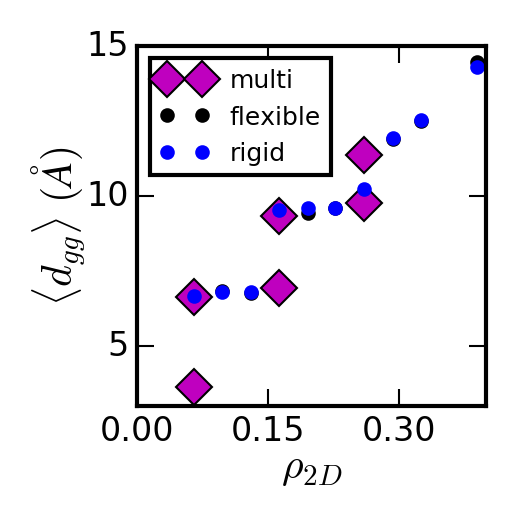
\includegraphics[trim={0.35cm 0.25cm 0.05cm 0.05cm},clip,width=.99\textwidth]{d_gg}
  	\end{subfigure}
	\caption{\textit{Plot of average graphene-graphene separation as a function of 2D-number density.} Multi refers to the instances in the flexible case where coexistence between multiple numbers of water layers was observed.}
	\label{fig:dgg_1}
\end{figure}

\begin{figure}[ht!]
	%\centering
	\begin{subfigure}[b]{0.99\textwidth}
    		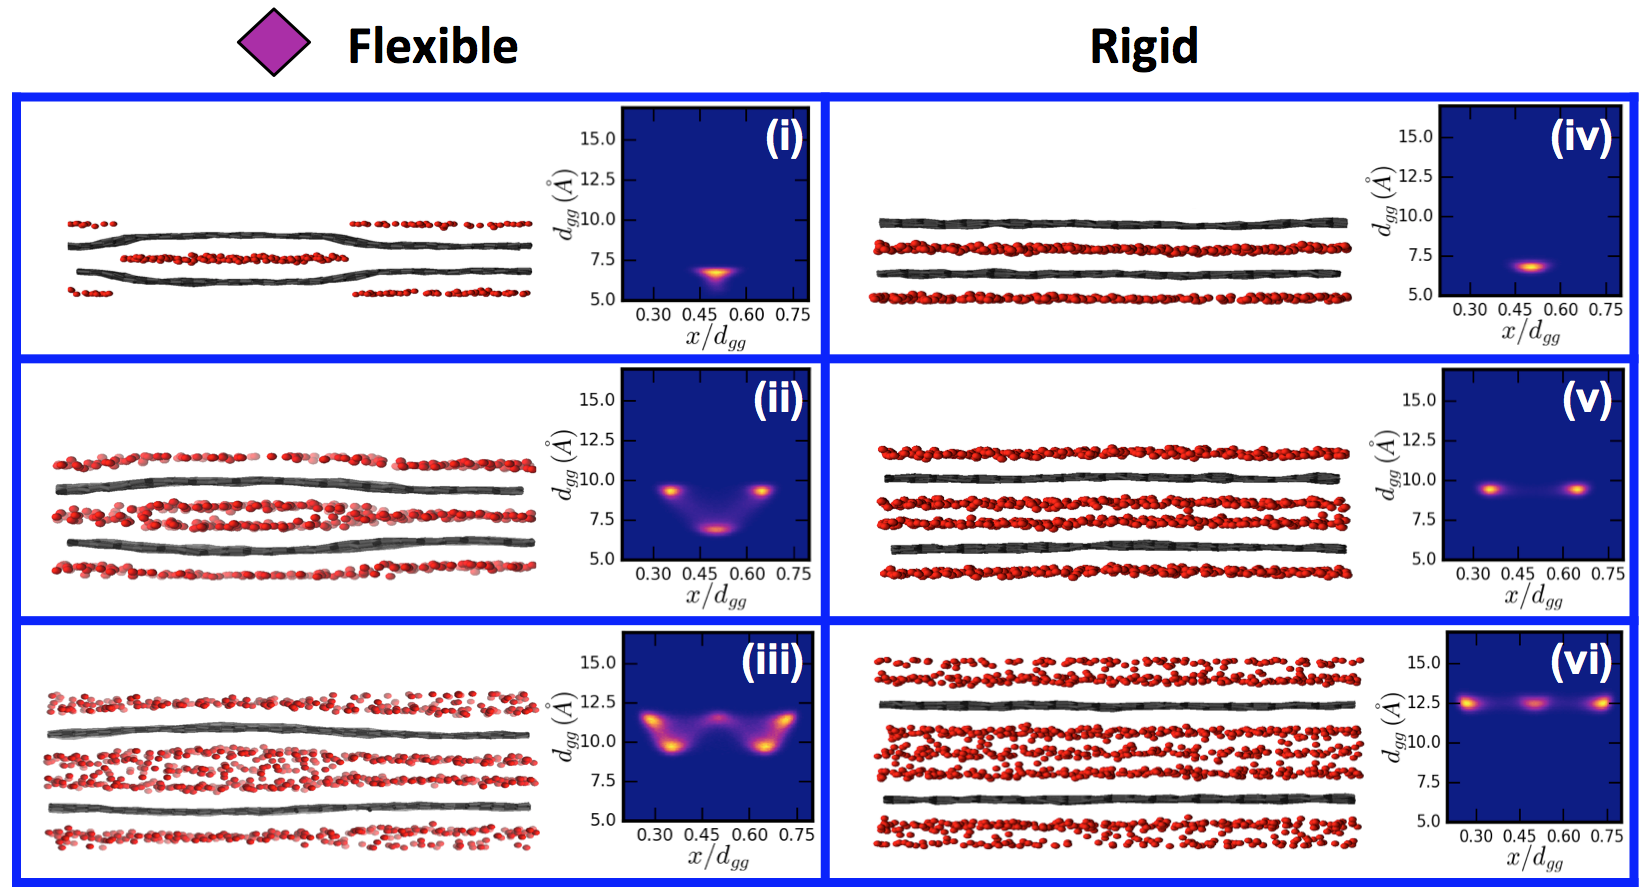
\includegraphics[width=.99\textwidth]{dgg_snaps7}
  	\end{subfigure}
	\caption{\textit{Snapshots of out-of-plane water layering and heatmap of water location and graphene-graphene separation.} \textbf{Snapshots.} Water-graphene systems as a function of increasing 2D-density, water oxygens are red, graphene carbons are grey and water hydrogens are not displayed for clarity. Panels (i), (ii) and (iii) correspond to flexible systems, and panels (iv), (v), and (vi) correspond to rigid systems. Images not drawn to size. \textbf{Heatmaps.} 2D histogram of the distance of water to a reference wall versus the graphene-graphene separation distance, warmer colors representing a higher number of observations.}
	\label{fig:dgg_2}
\end{figure}

\begin{figure}[ht!]
	\centering
	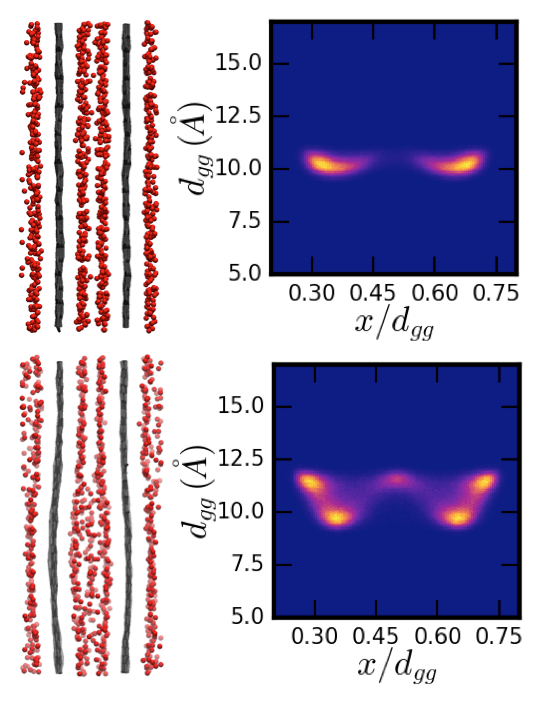
\includegraphics[trim={0.15cm 0.05cm 0.05cm 0.05cm},clip,width=0.49\textwidth]{d12_smearing} %
	\caption{\textit{Snapshots of out-of-plane water layering and heatmap of water location and graphene-graphene separation for bilayer to trilayer transition.} \textbf{Snapshots.} Water-graphene systems as a function of increasing 2D-density, water oxygens are red, graphene carbons are grey and water hydrogens are not displayed for clarity. Images not drawn to size. \textbf{Heatmaps.} 2D histogram of the distance of water to a reference wall versus the graphene-graphene separation distance, warmer colors representing a higher number of observations.}
	\label{fig:dgg_2_to_3}
\end{figure}


%%%%%%%%%%%%%%%%%%%%%%%%%%%%%%%%%%%%%%%%
%%%%%%%%%%%%%%%%%%%%%%%%%%%%%%%%%%%%%%%%

\textit{In-plane structure}. Besides the layering behavior illustrated in Figure \ref{fig:dgg_1} and Figure \ref{fig:dgg_2}, full characterization of the phases under confinement requires assessing the in-plane structure and dynamics of water, so we can discern among ice, liquid, gas, or more complicated behavior such as glass or heterogeneous liquid phases. In what follows, we review the change in behavior within each of the three regimes, namely from incomplete monolayer to full monolayer (\(\rho_{2D}=0.065\) to \(\rho_{2D}=0.097\)), from incomplete bilayer to full bilayer (\(\rho_{2D}=0.163\) to \(\rho_{2D}=0.196\)), and from incomplete trilayer to full trilayer (\(\rho_{2D}=0.260\) to \(\rho_{2D}=0.325\)), emphasizing the differences between rigid and flexible confinement.

 In the rigid case, as the density increased from 0.065 to 0.130, the RDF becomes substantially more structured (Fig \ref{fig:gr_ang_6_7_8_r}), which is also supported by the distributions of 3-body water oxygen intermolecular angles (Fig \ref{fig:gr_ang_6_7_8_r}), where there is a depopulation of intermediate (120-150 degrees) angles, and the distribution becomes clearly bimodal with peaks at 90 and 160 degrees, which are representative of square and rhombic ice. These ice structures are shown in Figure \ref{fig:ice_sq}. At the lowest 2D density, 0.063, there is not enough water to form a full monolayer, and the system becomes a mix of low-density gas and disordered liquid. As the density increases further, the low-density gas region disappears and the disordered liquid transitions to ice. This is also confirmed by trends in the lateral self-diffusion coefficient \(\mathcal{D}_{||}\), Figure \ref{fig:msd}. At the lowest density, \(\mathcal{D}_{||}\) is approximately that of bulk water, but this value drops by several orders of magnitude as density is increased to 0.130. 

In contrast to the rigid monolayer systems, the flexible monolayer systems display more variable properties due to the interaction between the variable density and the flexibility of the walls. At the lowest density, 0.063, the coexistence between 0 and 1 water layers eliminates the low density gas observed in the equivalent rigid system. Additionally, the pinned water region is highly structured ice, perhaps due to the lateral pressure of the graphene, an effect that has been previously observed and hypothesized (Ref \cite{Algara-Siller2015}). The high structure of this region is supported by RDF and 3-body angles (Fig \ref{fig:gr_ang_6_7_8_f}). As the density increases, the graphene walls flatten and the system is a mix of low density gas and  disordered liquid, much like the lowest 2D-density rigid system. At \(\rho_{2D}=0.130\), the flexible system becomes more structured and ice-like, similar to its rigid equivalent. Again, the transition from ice to liquid/gas and back to ice is confirmed by the variation in \(\mathcal{D}_{||}\) (Fig \ref{fig:msd}). The exact structure of these ice systems is examined in the next section. 

As density increases from 0.130 to 0.163, the systems transition from a monolayer to a bilayer system. In the rigid case, the bilayer forms a mixture of low density gas and ordered ice, at \(\rho_{2D}=\)0.163 and 0.196 (Fig \ref{fig:gr_ang_9_10_11_r}). The \(\mathcal{D}_{||}\) is orders of magnitude smaller than that of bulk water, confirming ice-like dynamics. The structure of this form of ice is discussed briefly in the next section. Finally, when density is increased to 0.227, this mixed structure disappears. The flexible system was not observed to form any ordered structure and was instead structurally similar to the rigid system at \(\rho_{2D}=\)0.227 (Fig \ref{fig:gr_ang_9_10_11_f}). It is interesting to note that in the flexible system with multi-water layer coexistence, two distinct RDFs were observed: one for water monolayer population and another for water in the bilayer. These distinct RDFs are included in Figure \ref{fig:gr_ang_9_10_11_f}.

Finally, as the density was increased beyond 0.260, less variation in in-plane structure is observed between the rigid and flexible systems, and is therefore not reported. Differences are observed in the computed \(\mathcal{D}_{||}\), Figure \ref{fig:msd}, but both display trends approaching bulk water with increasing density. \(\mathcal{D}_{||}\) values for the rigid systems are in good agreement with previous studies (Ref \cite{Mosaddeghi2012}), and the flexible trilayer values are generally larger than their rigid counterparts. 

% Mosaddeghi2012: 20A, D|| = 2.11, 15A, D|| = 0.95

\setlength{\fboxsep}{0.75pt}%
\setlength{\fboxrule}{1.2pt}%

\begin{figure}[ht!]
	\centering
	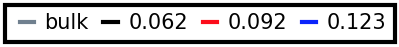
\includegraphics[width=0.46\textwidth]{leg_bulk_6_7_8}\\
  \fbox{\begin{subfigure}[b]{0.47\textwidth}
    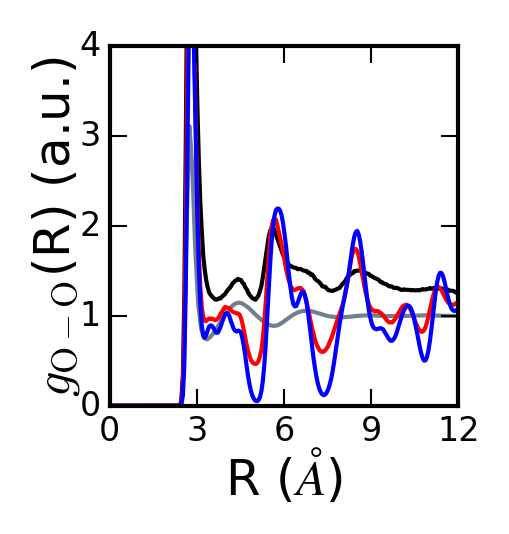
\includegraphics[trim={0.05cm 0.30cm 0.25cm 0.15cm},clip,width=0.46\textwidth]{g_r_2D_6_7_8_r}
    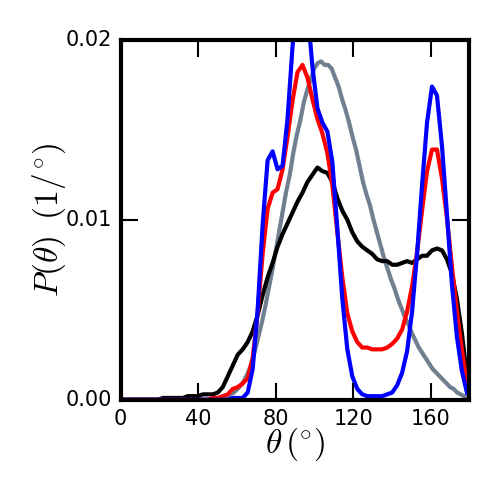
\includegraphics[trim={0.25cm 0.25cm 0.05cm 0.15cm},clip,width=0.485\textwidth]{ang_3B_6_7_8_r} 
     \fbox{\includegraphics[width=0.295\textwidth]{6A_r0} 
             	\llap{\raisebox{-0.4cm}{\color{white} \small  \fcolorbox{black}{black}{\(\mathcal{D}_{||}=2.26\)}}}}
     \fbox{\includegraphics[width=0.295\textwidth]{7A_r0}
     		\llap{\raisebox{-0.4cm}{\color{white} \small  \fcolorbox{red}{red}{\(\mathcal{D}_{||}=5.4e\scalebox{0.75}[1.0]{\( - \)}3\)}}}}
     \fbox{\includegraphics[width=0.295\textwidth]{8A_r0}
     		\llap{\raisebox{-0.4cm}{\color{white} \small  \fcolorbox{blue}{blue}{\(\mathcal{D}_{||}=1.4e\scalebox{0.75}[1.0]{\( - \)}4\)}}}}
    \caption{}
    \label{fig:gr_ang_6_7_8_r}
  \end{subfigure}}
  \fbox{\begin{subfigure}[b]{0.47\textwidth}
    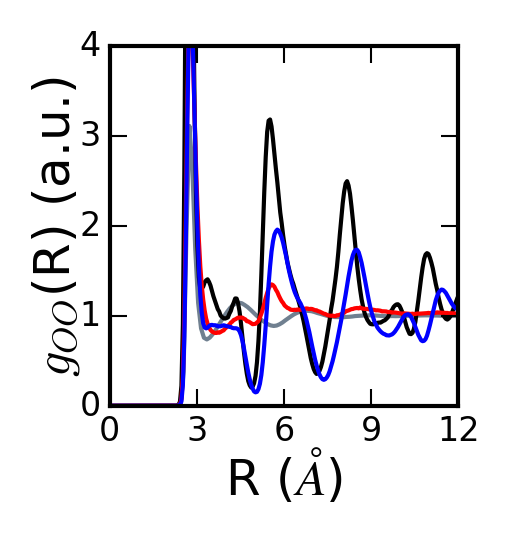
\includegraphics[trim={0.05cm 0.30cm 0.25cm 0.15cm},clip,width=0.46\textwidth]{g_r_2D_6_7_8_f}
    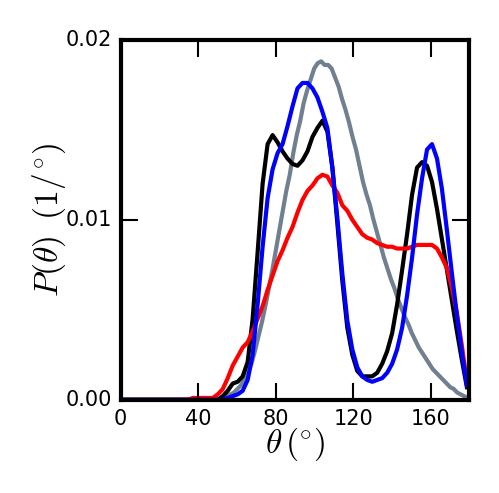
\includegraphics[trim={0.25cm 0.25cm 0.05cm 0.15cm},clip,width=0.485\textwidth]{ang_3B_6_7_8_f}
     \fbox{\includegraphics[width=0.295\textwidth]{6A_f0}
     		\llap{\raisebox{-0.4cm}{\color{white} \small \fcolorbox{black}{black}{\(\mathcal{D}_{||}=3.2e\scalebox{0.75}[1.0]{\( - \)}4\)}}}} %\raisebox{1.8cm} for in upper right corner
     \fbox{\includegraphics[width=0.295\textwidth]{7A_f0}
     		\llap{\raisebox{-0.4cm}{\color{white} \small \fcolorbox{red}{red}{\(\mathcal{D}_{||}=3.35\)}}}}
     \fbox{\includegraphics[width=0.295\textwidth]{8A_f0}
     		\llap{\raisebox{-0.4cm}{\color{white} \small \fcolorbox{blue}{blue}{\(\mathcal{D}_{||}=1.3e\scalebox{0.75}[1.0]{\( - \)}2\)}}}}
    \caption{}
    \label{fig:gr_ang_6_7_8_f}
  \end{subfigure}}
	\caption{\textit{Monolayer lateral oxygen-oxygen pair correlation functions, three-body angle distributions, and snapshots of monolayer systems.} (\protect\subref{fig:gr_ang_6_7_8_r}) rigid systems, (\protect\subref{fig:gr_ang_6_7_8_f}) flexible systems.  \textbf{Top.} Distribution of water oxygen distances and distribution of intralayer 3B angle formed between and given oxygen and its 2 nearest neighbors. \textbf{Bottom.} Snapshots of systems from left to right: \(\rho_{2D}=\) 0.065, 0.097, 0.130. Oxygens are in red, hydrogens are in white and for clarity, only one interlayer of water is depicted, and the graphene sheets are not displayed. Lateral diffusion coefficients are given in units of \((m^2/s) \times 10^9\), in the colored box in the bottom right corner. The lowest density system of (\protect\subref{fig:gr_ang_6_7_8_f}) is comprised of a coexistence between different number of water interlayers, highlighted in black (n=0) and blue (n=1).}
	\label{fig:struct_6_7_8}
\end{figure}

\begin{figure}[ht!]
	\centering
	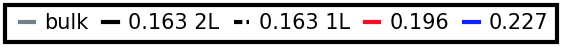
\includegraphics[width=0.60\textwidth]{leg_bulk_9_10_11}\\
  \fbox{\begin{subfigure}[b]{0.48\textwidth}
    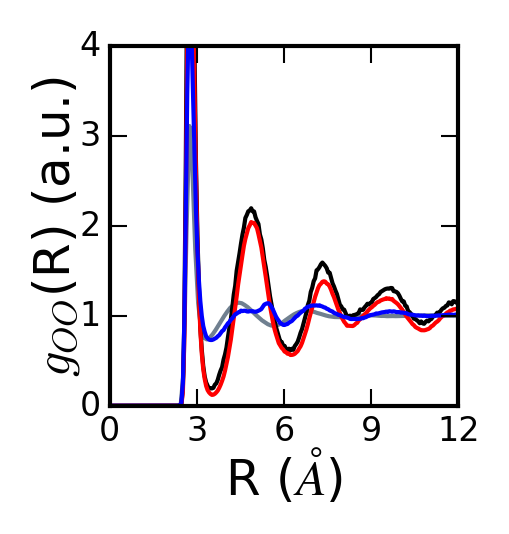
\includegraphics[trim={0.05cm 0.30cm 0.25cm 0.15cm},clip,width=0.46\textwidth]{g_r_2D_9_10_11_r}
    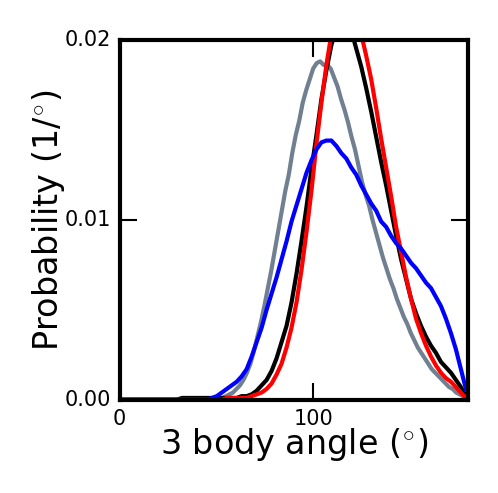
\includegraphics[trim={0.25cm 0.25cm 0.05cm 0.15cm},clip,width=0.485\textwidth]{ang_3B_9_10_11_r} 
     \fbox{\includegraphics[width=0.29\textwidth]{9A_r0}
     		\llap{\raisebox{-0.4cm}{\color{white} \small \fcolorbox{black}{black}{\(\mathcal{D}_{||}=2.2e\scalebox{0.75}[1.0]{\( - \)}2\)}}}}
     \fbox{\includegraphics[width=0.29\textwidth]{10A_r0}
     		\llap{\raisebox{-0.4cm}{\color{white} \small  \fcolorbox{red}{red}{\(\mathcal{D}_{||}=5.7e\scalebox{0.75}[1.0]{\( - \)}3\)}}}}
     \fbox{\includegraphics[width=0.29\textwidth]{11A_r0}
     		\llap{\raisebox{-0.4cm}{\color{white} \small  \fcolorbox{blue}{blue}{\(\mathcal{D}_{||}=1.07\)}}}}
    \caption{}
    \label{fig:gr_ang_9_10_11_r}
  \end{subfigure}}
  \fbox{\begin{subfigure}[b]{0.48\textwidth}
    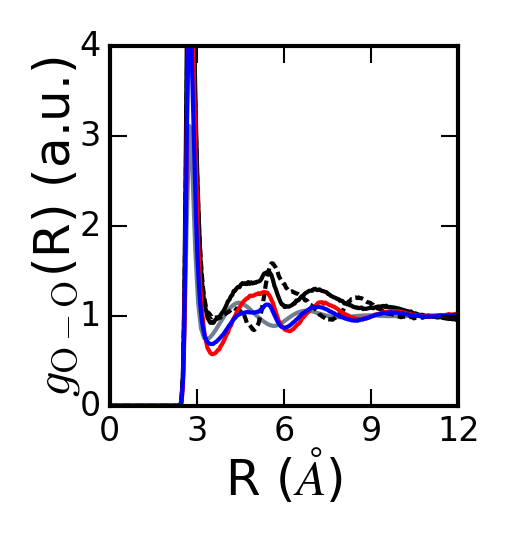
\includegraphics[trim={0.05cm 0.30cm 0.25cm 0.15cm},clip,width=0.46\textwidth]{g_r_2D_9_10_11_f}
    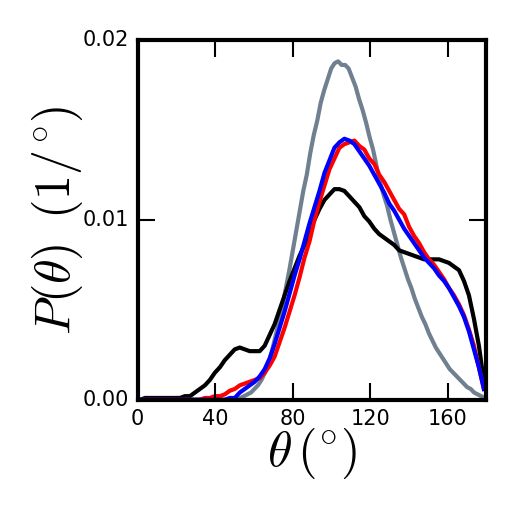
\includegraphics[trim={0.25cm 0.25cm 0.05cm 0.15cm},clip,width=0.485\textwidth]{ang_3B_9_10_11_f}
     \fbox{\includegraphics[width=0.29\textwidth]{9A_f0}
     		\llap{\raisebox{-0.4cm}{\color{white} \small  \fcolorbox{black}{black}{\(\mathcal{D}_{||}=1.79\)}}}}
     \fbox{\includegraphics[width=0.29\textwidth]{10A_f0}
     		\llap{\raisebox{-0.4cm}{\color{white} \small  \fcolorbox{red}{red}{\(\mathcal{D}_{||}=1.65\)}}}}
     \fbox{\includegraphics[width=0.29\textwidth]{11A_f0}
     		\llap{\raisebox{-0.4cm}{\color{white} \small  \fcolorbox{blue}{blue}{\(\mathcal{D}_{||}=1.22\)}}}}
    \caption{}
    \label{fig:gr_ang_9_10_11_f}
  \end{subfigure}}
	\caption{\textit{Bilayer lateral oxygen-oxygen pair correlation functions, three-body angle distributions, and snapshots of monolayer systems.} (\protect\subref{fig:gr_ang_9_10_11_r}) rigid systems, (\protect\subref{fig:gr_ang_9_10_11_f}) flexible systems. \textbf{Top.} Distribution of water oxygen distances and distribution of intralayer 3B angle formed between and given oxygen and its 2 nearest neighbors. \textbf{Bottom.} Snapshots of systems from left to right: \(\rho_{2D}=\) 0.163, 0.196, 0.227. Oxygens are in red, hydrogens are in white and for clarity, only one interlayer of water is depicted, and the graphene sheets are not displayed. Lateral diffusion coefficients are given in units of \((m^2/s) \times 10^9\), in the colored box in the bottom right corner. The lowest density system of (\protect\subref{fig:gr_ang_9_10_11_f}) is comprised of a coexistence between different number of water interlayers, highlighted in black (n=1) and blue (n=2).}
	\label{fig:struct_9_10_11}
\end{figure}

\begin{figure}[ht!]
	\centering
	\begin{subfigure}[b]{0.28\textwidth}
    		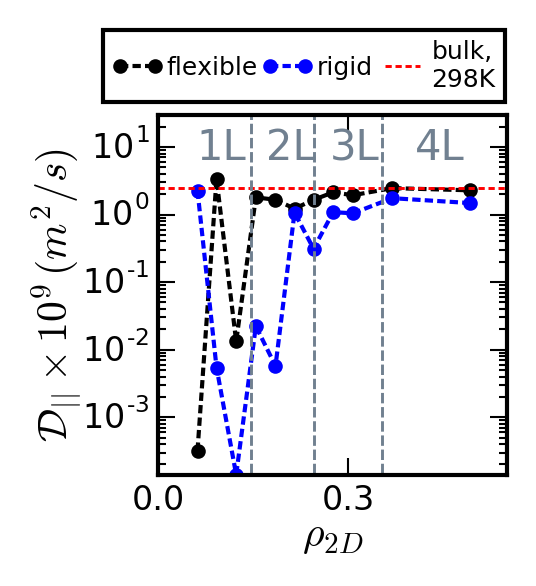
\includegraphics[trim={0.25cm 0.25cm 0.15cm 0.15cm},clip,width=0.99\textwidth]{diffusion_coeff_2D_f_r}
		\caption{}
    		\label{fig:diff}
   	\end{subfigure}	
	\begin{subfigure}[b]{0.28\textwidth}
    		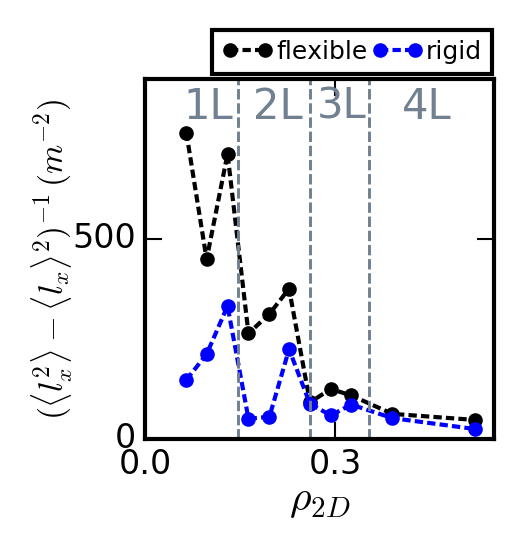
\includegraphics[trim={0.25cm 0.25cm 0.15cm 0.15cm},clip,width=0.99\textwidth]{compressibility}
		\caption{}
    		\label{fig:comp}
   	\end{subfigure}
	\caption{\textit{Comparison of dynamic properties}. (\protect\subref{fig:diff}) The self-diffusion coefficient as a function of number density for the diffusion parallel to the graphene walls. (\protect\subref{fig:comp}) Fluctuations in the out-of-plane distance as an approximation of system compressibility.}
	\label{fig:msd}
\end{figure}

%%%%%%%%%%%%%%%%%%%%%%%%%%%%%%%%%%%%%%%%
%%%%%%%%%%%%%%%%%%%%%%%%%%%%%%%%%%%%%%%%
\textit{Ice structure}.

\begin{figure}[ht!]
	\centering
	\begin{subfigure}[b]{0.395\textwidth}
    		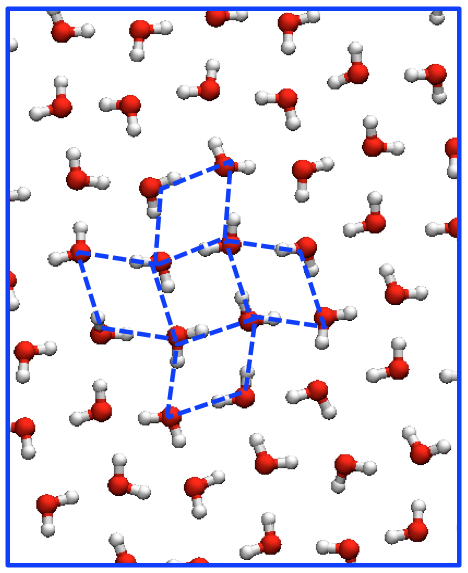
\includegraphics[width=.99\textwidth]{ice_square}
		\caption{}
        		\label{fig:ice_sq}
  	\end{subfigure}
	\begin{subfigure}[b]{0.285\textwidth}
    		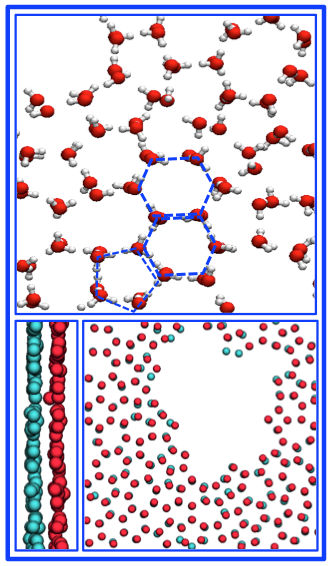
\includegraphics[width=.99\textwidth]{ice_hex}
		\caption{}
        		\label{fig:ice_hx}
  	\end{subfigure}
	\caption{\textit{Snapshots of the ice forms observed.} Oxygens are in red and cyan, hydrogens are in white. (\protect\subref{fig:ice_sq}) Square and off-square ice observed in the following monolayer systems: \(\rho_{2D}=\)0.065 (flexible), \(\rho_{2D}=\)0.097 (rigid), \(\rho_{2D}=\)0.130 (both). (\protect\subref{fig:ice_hx}) Hexagonal ice, observed in \(\rho_{2D}=\)0.163 and 0.196 (rigid). The top figure is a snapshot of the in-plane ordering. On the bottom, the A-A stacking between layers is highlighted by depicting the oxygens of each layer in red and cyan. Hydrogens are not pictured.}
	\label{fig:ice_figs}
\end{figure}

\clearpage
\printbibliography
\end{document}

\clearpage

\begin{figure}[ht!]
	\centering
	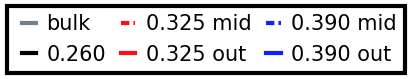
\includegraphics[width=0.60\textwidth]{leg_bulk_12_14_16}\\
  \fbox{\begin{subfigure}[b]{0.48\textwidth}
    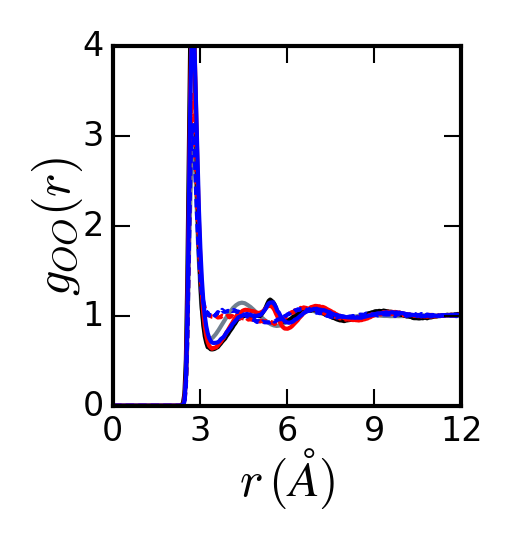
\includegraphics[trim={0.05cm 0.30cm 0.25cm 0.15cm},clip,width=0.46\textwidth]{g_r_2D_12_14_16_r}
    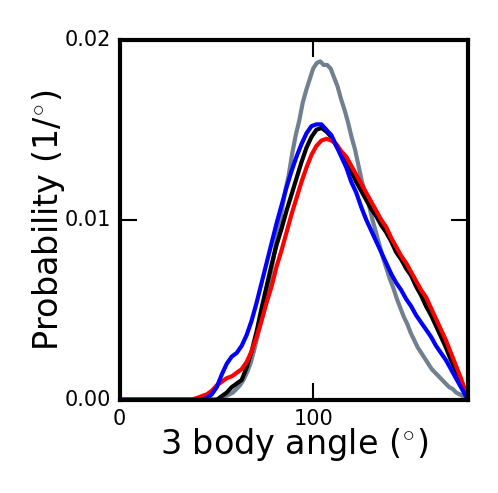
\includegraphics[trim={0.25cm 0.25cm 0.05cm 0.15cm},clip,width=0.485\textwidth]{ang_3B_12_14_16_r} 
     \fbox{\includegraphics[width=0.30\textwidth]{12A_r2}}
     \fbox{\includegraphics[width=0.30\textwidth]{14A_r3} }
     \fbox{\includegraphics[width=0.30\textwidth]{16A_r4}}
    \caption{}
    \label{fig:gr_ang_12_14_16_r}
  \end{subfigure}}
  \fbox{\begin{subfigure}[b]{0.48\textwidth}
    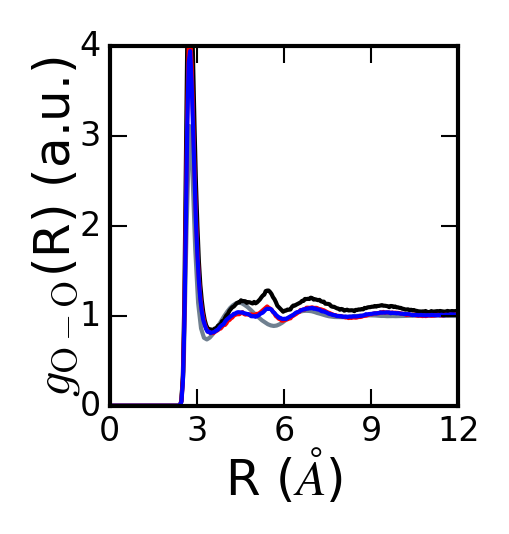
\includegraphics[trim={0.05cm 0.30cm 0.25cm 0.15cm},clip,width=0.46\textwidth]{g_r_2D_12_14_16_f}
    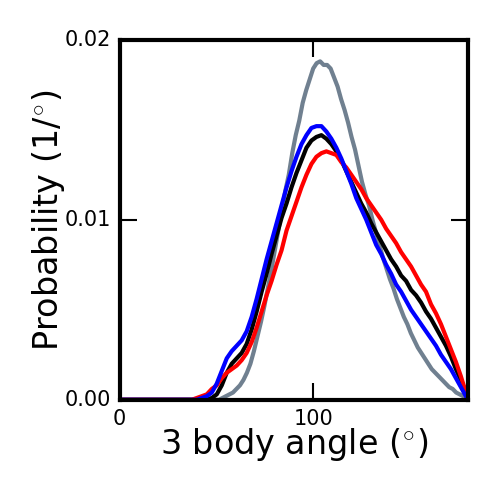
\includegraphics[trim={0.25cm 0.25cm 0.05cm 0.15cm},clip,width=0.485\textwidth]{ang_3B_12_14_16_f}
     \fbox{\includegraphics[width=0.31\textwidth]{12A_f2}}
     \fbox{\includegraphics[width=0.305\textwidth]{14A_f3}}
     \fbox{\includegraphics[width=0.305\textwidth]{16A_f3}}
    \caption{}
    \label{fig:gr_ang_12_14_16_f}
  \end{subfigure}}
	\caption{\textit{Trilayer lateral oxygen-oxygen pair correlation functions, three-body angle distributions, and snapshots of monolayer systems.} (\protect\subref{fig:gr_ang_12_14_16_r}) rigid systems, (\protect\subref{fig:gr_ang_12_14_16_f}) flexible systems. \textbf{Top.} Distribution of water oxygen distances and distribution of intralayer 3B angle formed between and given oxygen and its 2 nearest neighbors. \textbf{Bottom.} Snapshots of systems from left to right: \(\rho_{2D}=\) 0.163, 0.196, 0.227. Oxygens are in red, hydrogens are in white and for clarity, only one interlayer of water is depicted, and the graphene sheets are not displayed.}
	\label{fig:struct_12_14_16}
\end{figure}


\cite{Maniwa2005} 2005, XRD and MD studies of CNTs with varying diameters (10.9 - 15.2 \r A). Found four different structures. 
Also the melting temperature of the ice changed as a function of CNT diameter.


\cite{Algara-Siller2015} 2015, TEM and MD of ice in between graphene monolayers - saw ice of 1, 2 and 3 monolayers (with TEM).
With MD (SPC/E water), graph sheets of 68X58 \r A, and separations of 6.5, 9.0 11.5 \r A. ** VDW pressure, for a cluster of water between
two sheets??

\cite{Zangi2003,Zangi2003_2} 2003, studies of freezing and melting water of monolayer and bilayer ice.


%% BENZENE STUFF

%The benzene parameters were taken from the OPLS-AA force field \cite{Jorgensen1996}.
%The atom type \#145 was used for benzene carbons and \#146 was used for benzene
%hydrogens. This is from the papers: J. Am. Chem. SOC. 1990, 112, 4168-4114 \cite{Jorgensen1990}.
%and J. Am. Chem. Soc. 1996, 118, 11225-11236  \cite{Jorgensen1996}.  
%
%Nonbonded parameters
%\#   AN AT   CHARGE     SIGMA    EPSILON 
%145 06 CA   -0.115     3.550     0.070     Benzene C - 12 site JACS,112,4768-90
%146 01 HA    0.115     2.420     0.030     Benzene H - 12 site  "
%
%For bonds and angles, the following parameters were taken from AMBER all-atom
%\cite{Weiner1986} (also from zarbi.chem.yale.edu/doc/par\_opls\_aam.inp)
%Which has different CA-HA, and angle params.
%
%Bonds
%CA-CA 469.       1.40         TRP,TYR,PHE
%CA-HA 367.       1.080        PHE, etc. 
%
%Angles
%CA-CA-CA    63.        120.     PHE(OL)
%CA-CA-HA     35.       120.
%
%
%Torsions
%\#      v1        v2        v3       v4         notes
%165   0.0       7.250     0.0       0.0        CA-CA-CA-CA                           
%
%Improper
%improper\_coeff 1 1.1 -1 1  \# CA-CA-CA-HA for benzene 


\subsubsection*{Energy calculations}

The excess Gibbs free energy (G\textsubscript{excess}) of the confined water was calculated as the sum of the excess enthalpy (H\textsubscript{excess}) and the excess entropy (S\textsubscript{excess}) as follows:
\begin{equation}
    G\textsubscript{excess}  =  H_{\text{excess}} - T  S_{\text{excess}}
\end{equation}

Where is H\textsubscript{excess} defined as \textbf{\color{red}this is from \cite{Huggins2012}}. 
\begin{equation}
    H_{\text{excess}} = E_{\text{interaction}} - RT
\end{equation}

Where E\textsubscript{excess} is computed from long-range and pair interactions. Bonded energetics (bond stretching, angle bending) are not included because the water mode is rigid. Calculations of the excess entropy are detailed in the next section and have been taken from the method detailed by Huggins \cite{Huggins2012}.

\subsubsection*{Entropy calculations}

The molecular pair correlation function in water is a function of five angles and the intermolecular separation, as depicted in Figure \textbf{\color{red}OMG figure}. Using the pair correlation function, the excess entropy can be calculated as:
\begin{equation}
    S_{\text{excess}} = - \frac{1}{2} k_B \rho \int_V [ g(r, \omega) ln \, g(r, \omega) - g(r, \omega) + 1 ] d \mathbf{r} \, d\omega
\end{equation}
Where k\textsubscript{B} is Boltzmann's constant, \(\rho\) is the number density of bulk water and \(g(r, \omega)\) is the correlation function. This entropy is further divided into translational (S\textsubscript{trans}) and orientational (S\textsubscript{or}) components:
\begin{equation}
    S_{\text{excess}} = S_{\text{trans}} + S_{\text{or}}
\end{equation}
For this notation it is useful to separated the correlation function into a angle independent component and a conditional probability of the angles:
\begin{equation}
    g(r, \omega) = g(r) g(\omega | r)
\end{equation}
Now S\textsubscript{trans} and S\textsubscript{or} are written as follows:
\begin{equation}
    S_{\text{trans}} = - \frac{1}{2} k_B \rho \int_V [ g(r) ln \,  g(r) - g(r) + 1 ] d \mathbf{r} 
\end{equation}
\begin{equation}
   \begin{split}
    S_{\text{trans}} = & - \frac{1}{2} k_B \rho \int_0^\pi sin \theta d \theta \int_0^{2\pi} d \phi \int_0^\infty   [ g(r) ln\,  g(r) - g(r) + 1 ] r^2 dr \\
     = &  - {2} \pi k_B \rho \int_0^\infty   [ g(r) ln \,  g(r) - g(r) + 1 ] r^2 dr 
  \end{split}
\end{equation}
And the orientation component integrates over all five angles as a conditional probability of pair distance (r). The five angles contain symmetry such that the integration ranges are modified as given in Table \ref{table:ent_angles}.
\begin{table}[ht!]
\centering
\begin{tabular}{|c|r|r|}
\hline
\textbf{Angle} & \multicolumn{1}{c|}{\textbf{Original Range}} & \multicolumn{1}{c|}{\textbf{Actual Range}} \\ \hline
\( \theta_1\) & \([0, \pi]\)                             & \([0, \pi]\)                           \\ \hline
\( \theta_2\) & \([0, \pi]\)                             & \([0, \pi]\)                           \\ \hline
\( \chi_1\)   & \([0, 2\pi]\)                            & \([0, \pi]\)                           \\ \hline
\( \chi_2\)   & \([0, 2\pi]\)                            & \([0, \pi]\)                           \\ \hline
\( \phi\)      & \([0, 2\pi]\)                            & \([0, \pi]\)                           \\ \hline
\end{tabular}
\caption{\textit{Range of angles for five Euler angles of pair distribution functions.} The first column is the range used for full scheme, the second column is actual range used due to the symmetry of water.}
\label{table:ent_angles}
\end{table}
\begin{equation}
 \begin{split}
    S_{\text{or}} = & - \frac{1}{2} k_B \rho \int_V g(r) S_{\text{shell}} (r) d \textbf{r} \\
                        = & - \frac{1}{2} k_B \rho \int_0^\pi sin \theta d \theta \int_0^{2\pi} d \phi \int_0^\infty g(r) S_{\text{shell}} (r) r^2 dr
\end{split}
\end{equation}
Where S\textsubscript{shell} is given as:
\begin{equation}
    S_{\text{shell}} = \frac{1}{\Omega} \int g(\omega | r) ln \, g(\omega | r) d\omega
\end{equation}
Where the integrand (\( \int d\omega\)) is:
\begin{equation}
 \begin{split}
    \int d\omega & = \int sin \, \theta_1 d \theta_1 sin \, \theta_2 d \theta_2 d\phi_1 d\phi_2 d\chi_1 d\chi_2 \\
        & =  2\pi \int_0^\pi sin \, \theta_1 d \theta_1 \int_0^\pi sin \, \theta_2 d \theta_2 \int_0^\pi d\phi\int_0^\pi d\chi_1 \int_0^\pi d\chi_2 
 \end{split}
\end{equation}
And \(\Omega\) is the integral over all angles:
\begin{equation}
    \Omega = 2\pi \int_0^\pi sin \, \theta_1 d \theta_1 \int_0^\pi sin \, \theta_2 d \theta_2 \int_0^\pi d\phi\int_0^\pi d\chi_1 \int_0^\pi d\chi_2 = 2 \pi * 2 * 2 * \pi * \pi * \pi = 8 \pi^4
\end{equation}
Although the \(2\pi\) before the integrand is ignored because it will cancel with the normalization. For each of the angles, the distribution function is normalized such that:
\begin{equation}
    \frac{1}{\Omega} \int g(\omega | r ) \, d \omega = 1  
\end{equation}




